% ======================================================================
% ARTIGO_CRATEUS_RBEP.tex — Versão LaTeX do artigo (RBEP/INEP)
% Estudo Crateús-IDEB (R426): padrão associativo renda × IDEB na
% microrregião do Sertão de Cratéus (CE), com validações espelhadas.
% Compilar: pdflatex ARTIGO_CRATEUS_RBEP.tex (duas passadas)
% ======================================================================
\documentclass[12pt,a4paper]{article}

\usepackage[T1]{fontenc}
\usepackage[utf8]{inputenc}
\usepackage[brazilian]{babel}
\usepackage{newtxtext,newtxmath}
\usepackage[margin=3cm,top=3cm,left=3cm,right=2cm,bottom=2cm]{geometry}
\usepackage{setspace}
\usepackage{booktabs}
\usepackage{array}
\usepackage{graphicx}
\usepackage{microtype}
\usepackage{xurl}
\usepackage[hidelinks]{hyperref}

\onehalfspacing
\setlength{\parindent}{1.25cm}
\setlength{\parskip}{0pt}

\begin{document}

% ----------------------------------------------------------------------
% Título e resumos
% ----------------------------------------------------------------------
\begin{center}
{\Large\bfseries Desenvolvimento educacional em microrregião do Semiárido cearense: o padrão associativo entre desempenho escolar e renda no Sertão de Cratéus}
\end{center}

\noindent\textbf{Autor:} Marcelo Claro Laranjeira --- ORCID: \href{https://orcid.org/0000-0001-8996-2887}{https://orcid.org/0000-0001-8996-2887}

\vspace{0.8cm}

\section*{Resumo}

Este estudo testa, na microrregião do Sertão de Cratéus (Ceará, IBGE 23018; nove municípios), a relação entre desempenho escolar (IDEB) e renda municipal em duas dimensões complementares: entre unidades (níveis) e dentro das unidades ao longo do tempo. Com dados oficiais e auditáveis (INEP, edições 2005--2025; IBGE, PIB municipal 2010--2021 e Censo Demográfico 2022) e protocolo de validação robusto (bootstrap por cluster, primeiras diferenças, efeitos fixos de município e ano com erros clusterizados, validação cruzada leave-one-out por município, MDES e TOST), encontramos: (i) correlação transversal moderada-forte entre IDEB e log do PIB per capita defasado ($r = 0{,}49$; IC95\% $[0{,}34; 0{,}64]$), replicada fora da amostra em 9/9 municípios (LOOCV mediana $r = 0{,}62$); (ii) associação dentro da unidade nula (primeiras diferenças $r = -0{,}05$, $p = 0{,}61$) e coeficiente de efeitos fixos não significativo mesmo com erros clusterizados por município ($\beta = 2{,}61$; IC95\% cluster $[-1{,}51; 6{,}73]$; $p = 0{,}18$); (iii) MDES de 5,71 pontos (cluster) e TOST não significativo, indicando não-detecção (não equivalência) dado o n municipal; e (iv) evidência de que a premissa de estagnação do IDEB não se sustenta com os dados mais recentes: os nove municípios atingiram a meta pactuada para 2021 e apresentaram ganho médio de 5,93 pontos (anos iniciais, 2007--2025), sem associação estatisticamente discernível entre ganho educacional e renda do responsável ($r = -0{,}14$; $p = 0{,}73$). Conclui-se que, no Sertão de Cratéus, a associação renda--desempenho é transversal (entre municípios) e não temporal (dentro dos municípios), enquanto o crescimento educacional observado não acompanha variações de renda municipal --- consistente com a literatura sobre políticas educacionais do Ceará, embora sem pretensão causal.

\noindent\textbf{Palavras-chave:} IDEB; renda; microrregião; Ceará; painel municipal; validação cruzada; efeitos fixos.

\section*{Abstract}

This study tests, in the Sertão de Cratéus microregion (Ceará state, Brazil; IBGE 23018; nine municipalities), the relationship between school performance (IDEB) and municipal income in two complementary dimensions: across units (levels) and within units over time. Using official auditable data (INEP, 2005--2025 editions; IBGE, municipal GDP 2010--2021 and 2022 Demographic Census) and a robust validation protocol (cluster bootstrap, first differences, municipality-and-year fixed effects with clustered errors, leave-one-out cross-validation by municipality, MDES and TOST), we find: (i) moderate-to-strong cross-sectional correlation between IDEB and lagged log GDP per capita ($r = 0.49$; 95\% CI $[0.34, 0.64]$), replicated out-of-sample in 9/9 municipalities (LOOCV median $r = 0.62$); (ii) null within-unit association (first differences $r = -0.05$, $p = 0.61$) and nonsignificant fixed-effects coefficient even with municipality-clustered errors ($\beta = 2.61$; 95\% clustered CI $[-1.51, 6.73]$; $p = 0.18$); (iii) MDES of 5.71 points (clustered) and nonsignificant TOST, indicating non-detection (not equivalence) given the municipal sample size; and (iv) evidence that the premise of IDEB stagnation does not hold in the most recent data: all nine municipalities met the pactuated target for 2021 and showed a mean gain of 5.93 points (early grades, 2007--2025), with no statistically discernible association between educational gain and household head income ($r = -0.14$; $p = 0.73$). In Sertão de Cratéus, the income--performance association is cross-sectional (between municipalities) rather than temporal (within municipalities), while observed educational growth does not track municipal income variation --- consistent with the literature on Ceará's education policies, with no causal claims.

\noindent\textbf{Keywords:} IDEB; income; microregion; Ceará; municipal panel; cross-validation; fixed effects.

% ----------------------------------------------------------------------
% Corpo
% ----------------------------------------------------------------------
\section{Introdução}

A relação entre renda e desempenho educacional é um dos temas mais persistentes da pesquisa em educação comparada. Hanushek e Woessmann (2015) demonstraram que o ``capital de conhecimento'' de uma nação --- medido por habilidades cognitivas, e não apenas por anos de escolaridade --- associa-se fortemente ao crescimento econômico de longo prazo. No Brasil, análises de avaliação em larga escala mostram desigualdades substanciais associadas ao nível socioeconômico (Cito; Marôco, 2026), e estudos multiníveis documentam o impacto associativo da pobreza sobre o IDEB (Duarte, 2013; Andrews; Vries, 2012).

Uma distinção analítica frequentemente negligenciada separa dois tipos de associação entre renda e desempenho escolar: a \textbf{transversal} (entre unidades: municípios mais ricos tendem a ter IDEB mais alto) e a \textbf{temporal} (dentro de uma mesma unidade: quando a renda de um município cresce, seu IDEB cresce?). A primeira é amplamente documentada; a segunda é mais incerta e raramente testada em pequenas escalas. Para o Semiárido brasileiro, onde a pobreza é estrutural e a política educacional estadual (regime de colaboração, alfabetização na idade certa) produziu ganhos notáveis de aprendizagem, essa distinção tem implicações práticas: se a associação for apenas transversal, políticas de crescimento econômico local não deveriam ser tratadas como condição necessária para o avanço educacional.

A microrregião do Sertão de Cratéus (IBGE 23018), no Ceará, oferece um contexto privilegiado para esse teste: nove municípios pequenos, de baixa renda, sob a mesma coordenação estadual de políticas educacionais, com série histórica completa do IDEB (2005--2025) e indicadores municipais oficiais de renda (PIB municipal e Censo Demográfico 2022).

\textbf{Pergunta de pesquisa (RQ):} no Sertão de Cratéus, a associação entre renda municipal e desempenho escolar no IDEB é transversal (entre municípios), temporal (dentro dos municípios), ou ambas? Em particular: (a) municípios com maior renda têm IDEB mais alto? (b) variações de renda dentro do município acompanham variações de IDEB? (c) o ganho educacional observado na região depende da renda municipal, e os municípios cumprem as metas pactuadas pelo INEP?

Deliberadamente, este estudo não testa causalidade: trata-se de evidência associativa, com descrição explícita dos limites de inferência. As hipóteses operacionalizadas na Seção 3 respondem diretamente à RQ.

\section{Fundamentação}

\subsection{O IDEB como indicador e política}

O IDEB, criado em 2007, combina fluxo escolar e proficiência no SAEB, atribuindo metas bianuais às escolas públicas (Soares; Xavier, 2013; Schneider; Nardi, 2014). A literatura critica seu caráter de accountability gerencial (Afonso, 2012), mas reconhece sua função mobilizadora (Lacruz; Américo; Carniel, 2019). Brunello e Kiss (2022) mostram, em contexto internacional, que avaliações com consequências (``high stakes'') alteram o comportamento de escolas e professores.

\subsection{O caso do Ceará: regime de colaboração e alfabetização}

O Ceará tornou-se caso emblemático por seu regime de colaboração entre estado e municípios, institucionalizado pelo Programa Alfabetização na Idade Certa (PAIC, Lei 14.026/2007). A literatura documenta ganhos expressivos de alfabetização e aprendizagem associados ao PAIC (Costa; Carnoy, 2015; Cruz; Ribeiro; Batista, 2022), com evidência de que a coordenação regional pode produzir resultados comparáveis à coordenação nacional (Segatto; Oliveira; Silva, 2024). Carnoy et al.\ (2017) mostraram, em análise intranacional, que diferenças estaduais de desempenho no Brasil podem ensinar sobre políticas eficazes --- e o Ceará figura entre os casos de maior progresso.

\subsection{Renda e desempenho: associação transversal vs.\ temporal}

Em análises transversais, municípios mais ricos tendem a apresentar IDEB mais alto (Duarte, 2013; Andrews; Vries, 2012). Contudo, dentro de uma mesma unidade ao longo do tempo, a variação da renda não costuma acompanhar a variação do desempenho --- o crescimento do IDEB frequentemente ocorre mesmo onde a renda cresce pouco, como documentado para municípios pobres brasileiros (Andrews; Vries, 2012). Esse contraste entre associação transversal (em níveis) e ausência de associação temporal (dentro das unidades) fundamenta a distinção operacional deste estudo: medir separadamente as duas dimensões na mesma microrregião, em vez de combiná-las em um único coeficiente.

\section{Método}

\subsection{Delimitação e dados}

A microrregião do Sertão de Cratéus (IBGE 23018) compreende nove municípios: Ararendá (2301257), Crateús (2304103), Independência (2305605), Ipaporanga (2305654), Monsenhor Tabosa (2308609), Nova Russas (2309300), Novo Oriente (2309409), Quiterianópolis (2311264) e Tamboril (2313203). Usaram-se apenas fontes oficiais e auditáveis:

\begin{itemize}
\item \textbf{INEP --- IDEB municipal}, edição 2025 (série 2005--2025), rede Municipal, anos iniciais e finais do ensino fundamental (download.inep.gov.br);
\item \textbf{IBGE --- PIB dos Municípios}, base 2010--2021 (ftp.ibge.gov.br), PIB per capita a preços correntes;
\item \textbf{IBGE --- Censo Demográfico 2022}, agregados por município: rendimento nominal médio mensal das pessoas responsáveis (V06004) e mediana (V06006);
\item \textbf{IBGE --- Malha municipal 2023} (geoftp), para os mapas.
\end{itemize}

Todos os downloads foram registrados em manifesto de proveniência (URL, timestamp, SHA-256), disponível em \texttt{data/raw/SOURCE\_MANIFEST.json}. O IPCE (IPC Marketing Editora), mencionado na demanda original, é um índice comercial sem acesso público auditável; portanto, usaram-se como proxies oficiais o PIB per capita e a renda do responsável, com essa limitação declarada.

\subsection{Painel e variáveis}

O painel emparelha, por município e ano, o IDEB observado ao log do PIB per capita defasado em dois anos (IDEB do ano $t$ com PIB de $t-2$), suavizando contemporaneidade mecânica. Para a microrregião, o painel de estimação cobre os anos IDEB 2013--2023 ($n = 108$ observações; 9 municípios $\times$ 6 anos $\times$ 2 etapas). Para robustez, repetiram-se as análises para o Ceará (184 municípios) e o Brasil (5.360 municípios).

\subsection{Hipóteses}

\begin{itemize}
\item \textbf{H1 (níveis):} a correlação transversal entre IDEB e log do PIB per capita é positiva e estatisticamente discernível ($r \geq 0{,}3$; IC95\% sem 0).
\item \textbf{H2 (dentro):} a associação dentro das unidades é fraca ou nula --- primeiras diferenças $r$ próximo de zero e coeficiente de efeitos fixos de município e ano não significativo.
\item \textbf{H3 (estagnação):} o ganho de IDEB (2007 até o último disponível) é inferior à meta pactuada pelo INEP (VL\_PROJECAO\_2021) e não se associa à renda municipal.
\end{itemize}

\subsection{Procedimentos de validação}

\begin{enumerate}
\item \textbf{Correlações em níveis:} Pearson com intervalo de confiança por bootstrap por cluster (município), seed 42, 2.000 réplicas (500 quando o número de clusters excede 50).
\item \textbf{Primeiras diferenças:} correlação de Pearson das diferenças de primeira ordem dentro de cada município-etapa.
\item \textbf{Efeitos fixos:} regressão com efeitos fixos de município e ano via within-transformation dupla (município e ano). Reportam-se erros padrão homocedásticos (transparência) e \textbf{erros padrão clusterizados por município} (CRVE com correção de pequena amostra, $t$ com $G-1$ graus de liberdade).
\item \textbf{LOOCV por município:} para cada um dos nove municípios, estima-se a correlação nos oito restantes e avalia-se a replicação no município retido, reportando a distribuição dos $r$ de teste.
\item \textbf{MDES/TOST:} mínimo efeito detectável (poder 80\%, $\alpha$ 5\%) e teste de equivalência com margem $\pm 0{,}10$ no coeficiente de efeitos fixos, ambos baseados no erro padrão clusterizado ($G-1$ graus de liberdade).
\item \textbf{Transparência:} os scripts \path{baixar_dados.py}, \path{analise_crateus.py} e \path{mapa_crateus.py} estão na pasta \texttt{scripts/}. Saídas completas em \path{outputs/expanded/resultados_r426.json} e \path{provenance_r426.json}.
\end{enumerate}

\subsection{Critérios de invalidação empírica (falsificabilidade)}

Para que as hipóteses sejam testáveis, cada uma tem critérios de rejeição pré-definidos, passíveis de refutação pelos dados:

\begin{itemize}
\item \textbf{H1 seria rejeitada} se o IC95\% do bootstrap por cluster incluísse zero ou se a correlação transversal fosse negativa.
\item \textbf{H2 seria rejeitada} se o coeficiente de efeitos fixos (clusterizado) fosse estatisticamente discernível de zero ao nível de 5\% ou se as primeiras diferenças mostrassem correlação $|r| \geq 0{,}30$ com $p < 0{,}05$.
\item \textbf{H3 seria rejeitada} se a maioria dos municípios ($\geq 5$ de 9) ficasse abaixo da meta pactuada para 2021 ou se o ganho educacional correlacionasse positiva e significativamente com a renda municipal ($r > 0{,}30$; $p < 0{,}05$).
\end{itemize}

A não-detecção (MDES alto, TOST não significativo) é tratada como resultado informativo de poder estatístico, não como confirmação de ausência de efeito.

\section{Resultados}

\subsection{H1 --- associação em níveis}

Na microrregião, a correlação transversal entre IDEB e log do PIB per capita defasado foi $r = 0{,}49$ (IC95\% bootstrap por cluster $[0{,}34; 0{,}64]$; $p < 0{,}001$; $n = 108$; 9 clusters), confirmando H1. Para o Ceará, $r = 0{,}26$ (IC95\% $[0{,}20; 0{,}33]$); para o Brasil, $r = 0{,}46$ (IC95\% $[0{,}44; 0{,}47]$; $n = 48.695$). A associação em níveis está presente na microrregião, embora com magnitude moderada --- não tão elevada quanto a documentada em nível de países, mas consistente com a literatura municipal brasileira (Figura 1).

\begin{figure}[h!]
\centering
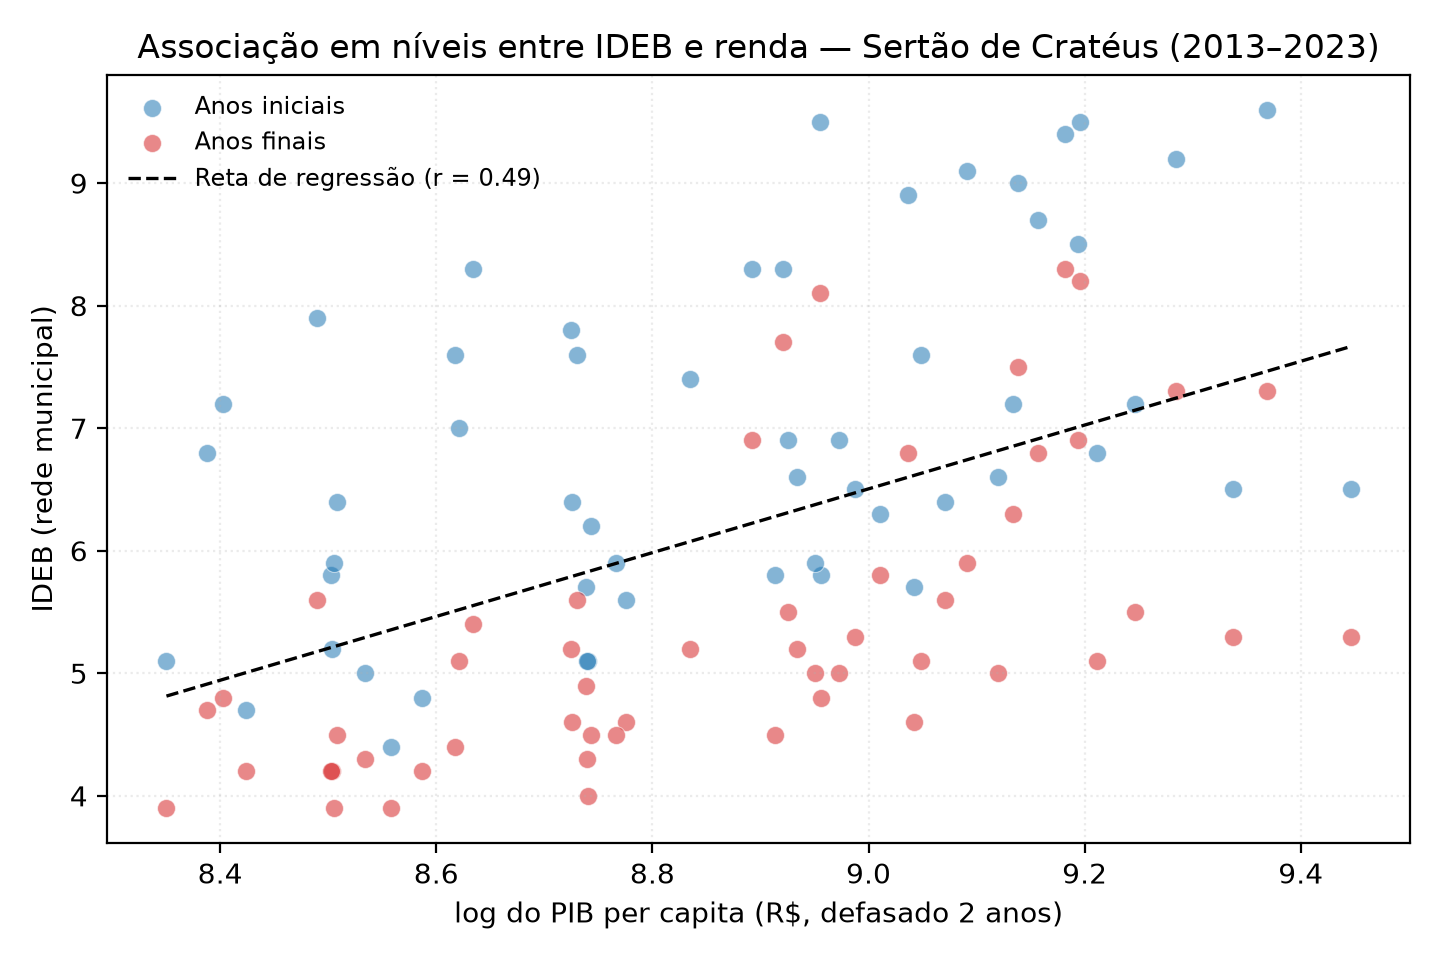
\includegraphics[width=0.72\textwidth]{../outputs/figuras/fig_scatter_niveis_micro.png}
\caption{Associação em níveis entre IDEB e log do PIB per capita (Sertão de Cratéus, 2013--2023), por etapa.}
\end{figure}

\begin{table}[h!]
\centering
\caption{Correlações em níveis por escala (IDEB $\times$ log do PIB per capita defasado)}
\small
\begin{tabular}{lcccc}
\toprule
\textbf{Escala} & \textbf{n} & \textbf{Clusters} & \textbf{r} & \textbf{IC95\% bootstrap} \\
\midrule
Microrregião Sertão de Cratéus & 108 & 9 & 0,49 & $[0{,}34; 0{,}64]$ \\
Ceará & 2.202 & 184 & 0,26 & $[0{,}20; 0{,}33]$ \\
Brasil & 48.695 & 5.360 & 0,46 & $[0{,}44; 0{,}47]$ \\
\bottomrule
\end{tabular}
\end{table}

\subsection{H2 --- associação dentro das unidades}

As primeiras diferenças dentro de município-etapa na microrregião foram nulas: $r = -0{,}05$ ($p = 0{,}61$; $n = 90$). O coeficiente de efeitos fixos de município e ano foi $\beta = 2{,}61$ (SE clusterizado 1,79; IC95\% cluster $[-1{,}51; 6{,}73]$; $p = 0{,}18$; $n = 108$): positivo, mas não estatisticamente discernível de zero, mesmo com erros clusterizados. Para o Ceará, $\beta = 0{,}001$ (IC95\% cluster $[-0{,}26; 0{,}26]$; $p = 0{,}99$). Para o Brasil, $\beta = 0{,}11$ (IC95\% cluster $[0{,}07; 0{,}15]$; $p < 0{,}001$): pequeno, embora discernível dado o enorme $n$. H2 se confirma na microrregião e no Ceará: dentro das unidades, a associação entre variação de renda e variação de IDEB não é discernível.

\begin{table}[h!]
\centering
\caption{Associação dentro das unidades por escala}
\small
\begin{tabular}{lcccc}
\toprule
\textbf{Escala} & \textbf{1\textordfeminine\ dif. r (p)} & \textbf{n (1\textordfeminine\ dif.)} & \textbf{FE $\beta$ (IC95\% cluster)} & \textbf{n (FE)} \\
\midrule
Microrregião Sertão de Cratéus & $-0{,}05$ (0,61) & 90 & $2{,}61$ ($[-1{,}51; 6{,}73]$) & 108 \\
Ceará & $0{,}03$ (0,27) & 1.834 & $0{,}001$ ($[-0{,}26; 0{,}26]$) & 2.202 \\
Brasil & $0{,}06$ (< 0,001) & 39.760 & $0{,}11$ ($[0{,}07; 0{,}15]$) & 48.695 \\
\bottomrule
\end{tabular}
\end{table}

\subsection{Validação cruzada leave-one-out por município}

A correlação de níveis estimada fora da amostra (treino nos oito municípios restantes, teste no município retido) foi positiva em 9/9 municípios (100\%), com mediana $r = 0{,}62$ (média 0,65; DP 0,11). Os $r$ de teste por município variaram de 0,43 (Quiterianópolis) a 0,81 (Ararendá). A associação em níveis não depende de um único município: é replicável em todos os nove (Figuras 2 e 3).

\begin{figure}[h!]
\centering
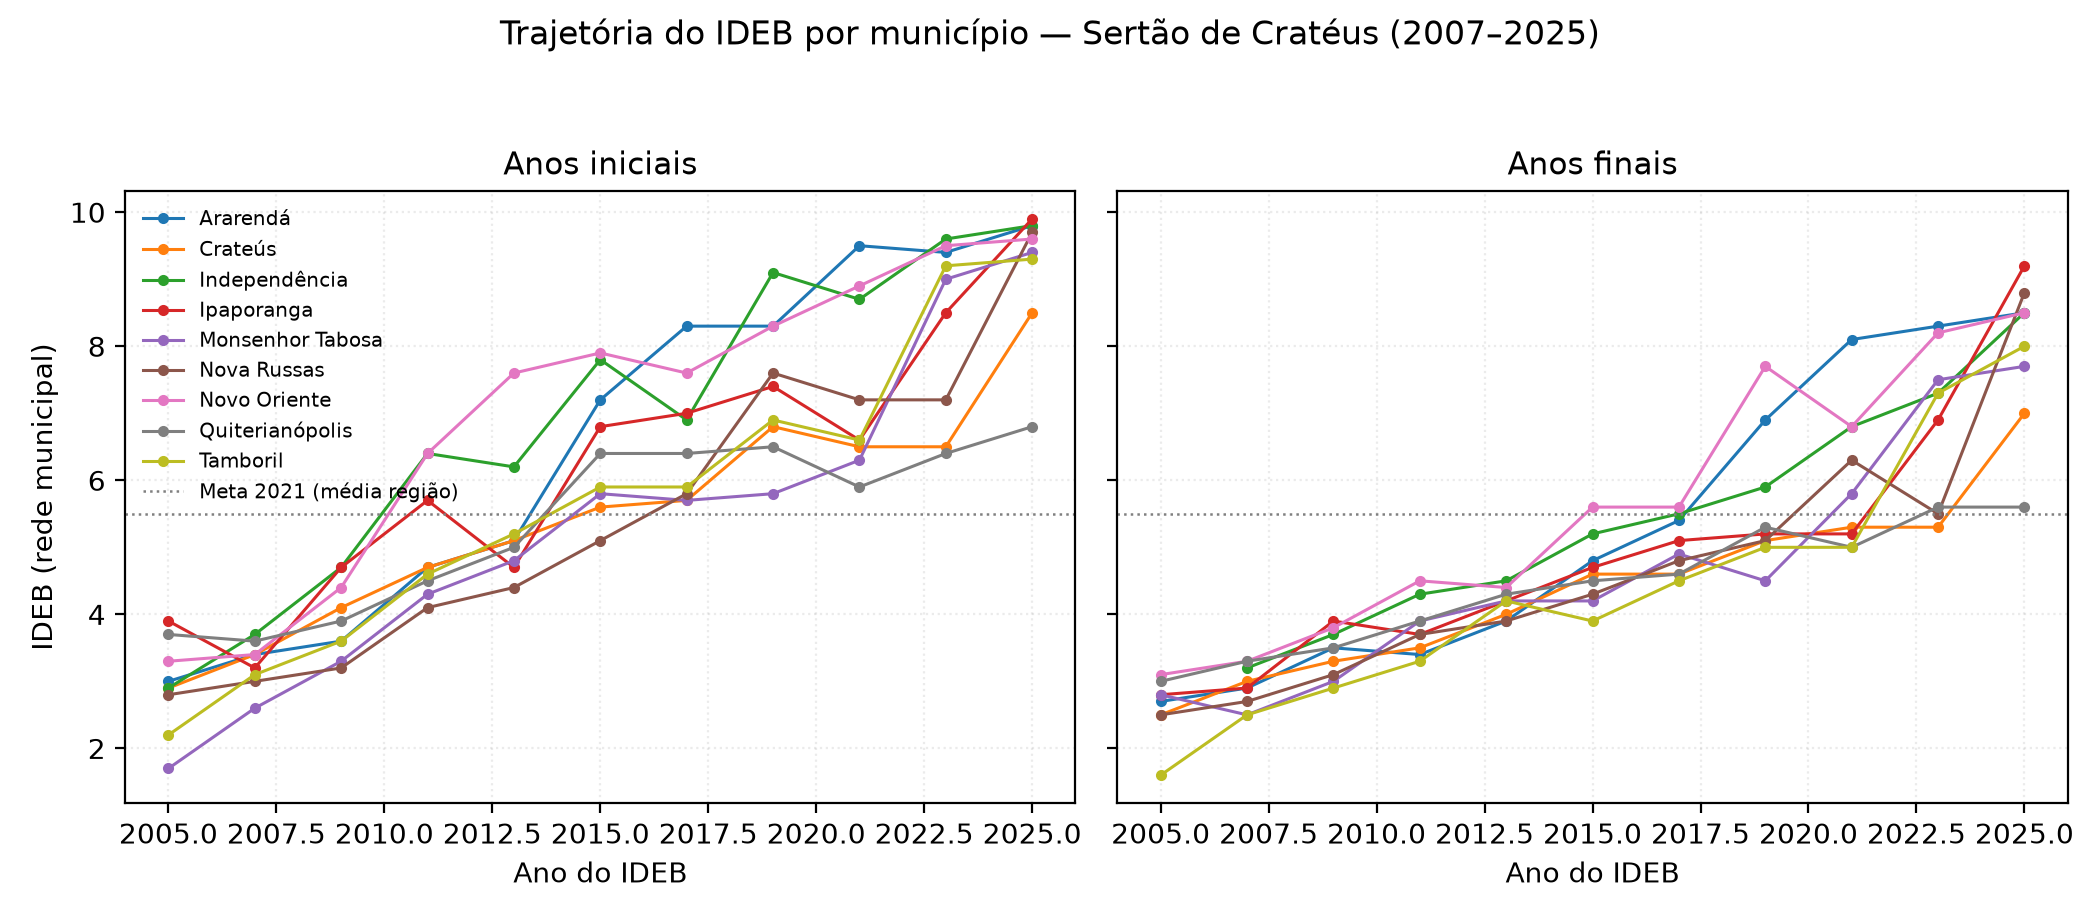
\includegraphics[width=0.98\textwidth]{../outputs/figuras/fig_serie_ideb_micro.png}
\caption{Trajetória do IDEB por município, 2007--2025 (anos iniciais e finais).}
\end{figure}

\begin{figure}[h!]
\centering
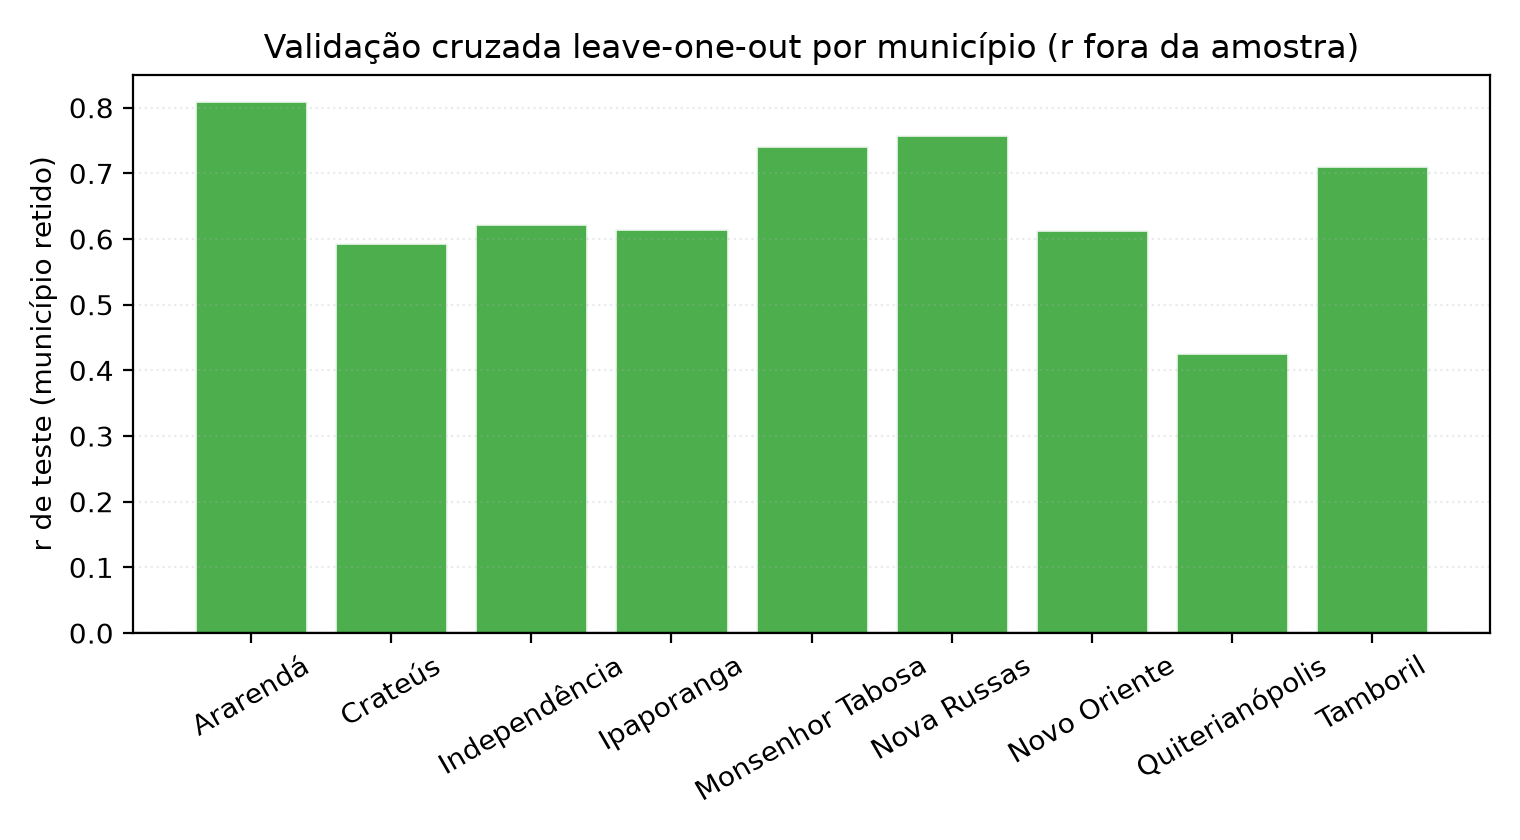
\includegraphics[width=0.72\textwidth]{../outputs/figuras/fig_loocv_r_teste.png}
\caption{Validação cruzada leave-one-out: $r$ de teste por município retido.}
\end{figure}

\begin{table}[h!]
\centering
\caption{Validação cruzada leave-one-out por município ($r$ de teste)}
\small
\begin{tabular}{lccc}
\toprule
\textbf{Município retido} & \textbf{r treino} & \textbf{r teste} & \textbf{n teste} \\
\midrule
Ararendá & 0,50 & 0,81 & 12 \\
Crateús & 0,57 & 0,59 & 12 \\
Independência & 0,46 & 0,62 & 12 \\
Ipaporanga & 0,48 & 0,62 & 12 \\
Monsenhor Tabosa & 0,46 & 0,74 & 12 \\
Nova Russas & 0,49 & 0,76 & 12 \\
Novo Oriente & 0,51 & 0,61 & 12 \\
Quiterianópolis & 0,49 & 0,43 & 12 \\
Tamboril & 0,46 & 0,71 & 12 \\
\bottomrule
\end{tabular}
\end{table}

\subsection{MDES e TOST}

Com n municipal de 9 e 108 observações, o mínimo efeito detectável foi de 5,71 pontos de IDEB por unidade de log do PIB (erro clusterizado, $G-1 = 8$ graus de liberdade; 6,05 com erro homocedástico) --- muito acima de qualquer coeficiente plausível. O teste de equivalência (TOST, margem $\pm 0{,}10$) não foi significativo ($p = 0{,}90$). Portanto, o correto é declarar \textbf{não-detecção}: a amostra não permite afirmar efeito, mas tampouco permite declarar equivalência. Essa é uma limitação central, explicitamente assumida.

\subsection{H3 --- ganho educacional e metas}

Contrariando a premissa de estagnação, os dados INEP 2025 mostram crescimento expressivo do IDEB nos nove municípios (anos iniciais, 2007--2025): ganho médio de 5,93 pontos, com todos os municípios \textbf{acima da meta pactuada para 2021}. O IDEB 2025 em anos iniciais variou de 6,8 (Quiterianópolis) a 9,9 (Ipaporanga), valores superiores à média nacional da rede municipal. Em anos finais, todos os nove municípios também atingiram a meta 2021. A correlação entre ganho de IDEB (anos iniciais) e renda média do responsável foi nula: $r = -0{,}14$ ($p = 0{,}73$; $n = 9$; Figura 4). Ou seja: não há evidência de que municípios com maior renda tenham tido maior ganho educacional --- o crescimento ocorreu de forma generalizada e não acompanhou a variação de renda.

\begin{figure}[h!]
\centering
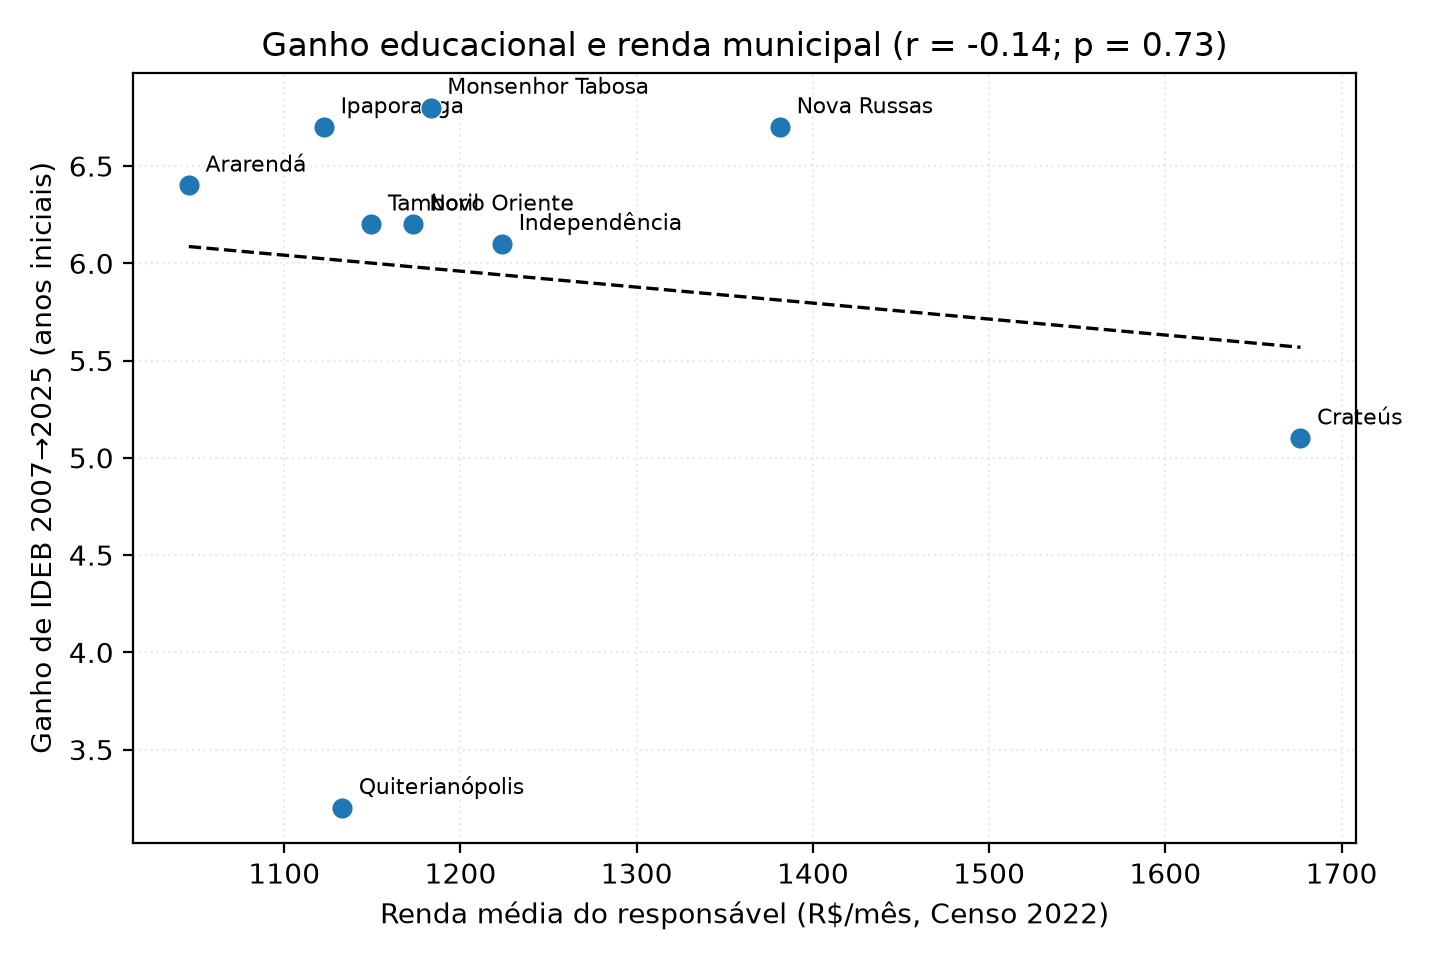
\includegraphics[width=0.72\textwidth]{../outputs/figuras/fig_scatter_ganho_renda.png}
\caption{Ganho de IDEB (2007--2025, anos iniciais) e renda média do responsável (Censo 2022).}
\end{figure}

\begin{table}[h!]
\centering
\caption{IDEB 2025, ganho 2007--2025 e meta 2021 (anos iniciais)}
\small
\begin{tabular}{lccccc}
\toprule
\textbf{Município} & \textbf{IDEB 2007} & \textbf{IDEB 2025} & \textbf{Ganho} & \textbf{Meta 2021} & \textbf{Atingiu meta} \\
\midrule
Ararendá & 3,4 & 9,8 & 6,4 & 5,3 & Sim \\
Crateús & 3,4 & 8,5 & 5,1 & 5,2 & Sim \\
Independência & 3,7 & 9,8 & 6,1 & 5,2 & Sim \\
Ipaporanga & 3,2 & 9,9 & 6,7 & 6,1 & Sim \\
Monsenhor Tabosa & 2,6 & 9,4 & 6,8 & 4,4 & Sim \\
Nova Russas & 3,0 & 9,7 & 6,7 & 5,1 & Sim \\
Novo Oriente & 3,4 & 9,6 & 6,2 & 5,6 & Sim \\
Quiterianópolis & 3,6 & 6,8 & 3,2 & 5,9 & Sim \\
Tamboril & 3,1 & 9,3 & 6,2 & 4,4 & Sim \\
\bottomrule
\end{tabular}
\end{table}

\subsection{Mapas}

Os mapas coropléticos (Figuras 5 e 6) apresentam os dois proxies oficiais de desenvolvimento por município: renda média mensal do responsável (Censo 2022, IBGE) e PIB per capita (2021, IBGE). Crateús, sede regional, destaca-se em ambos os indicadores; os demais municípios concentram-se nas faixas inferiores, retratando a heterogeneidade intra-regional que a análise transversal explora.

\begin{figure}[h!]
\centering
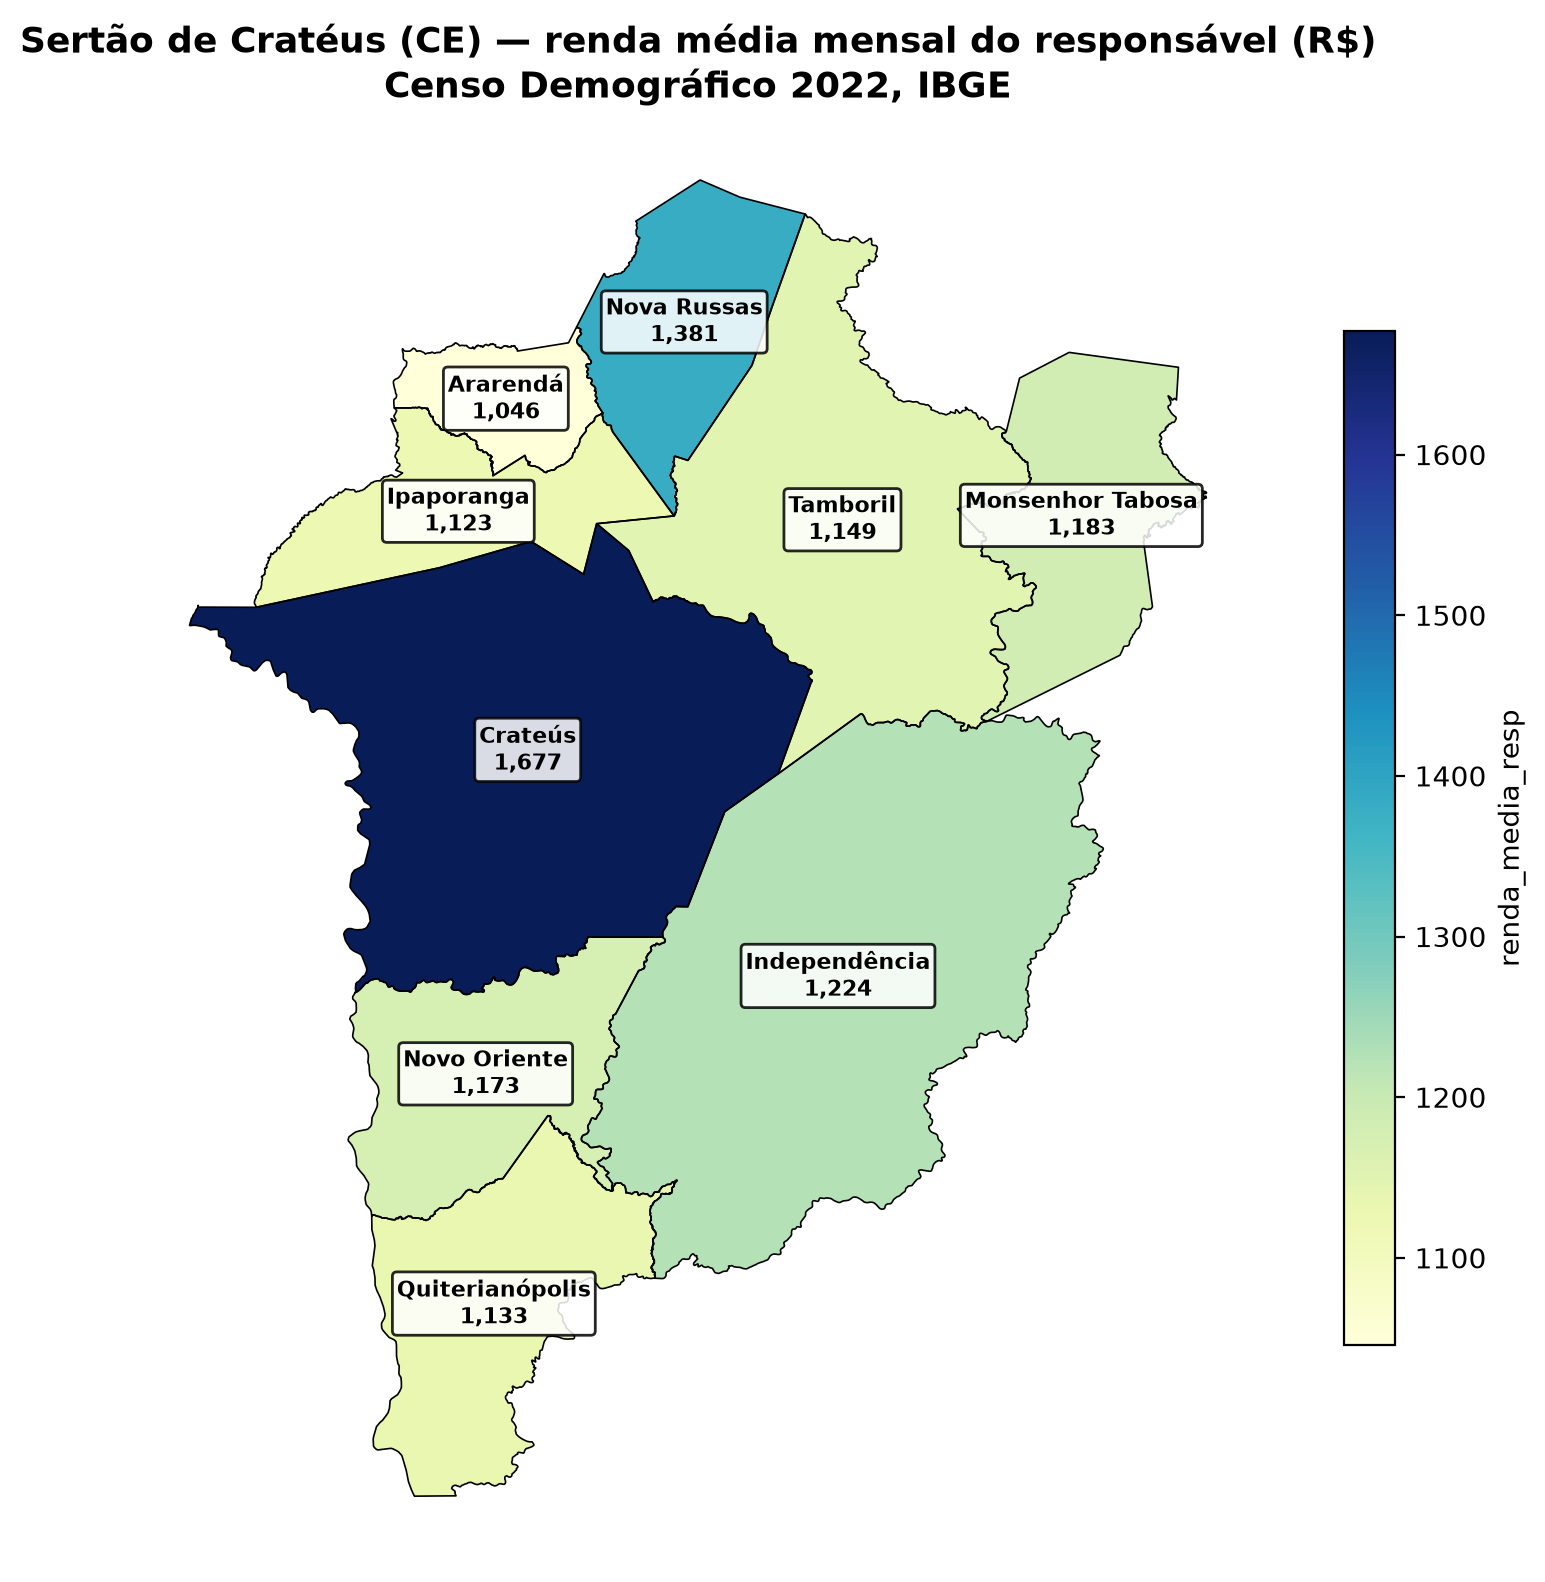
\includegraphics[width=0.78\textwidth]{../outputs/mapas/mapa_renda_responsavel_censo2022.png}
\caption{Renda média mensal do responsável por município (Censo 2022, IBGE).}
\end{figure}

\begin{figure}[h!]
\centering
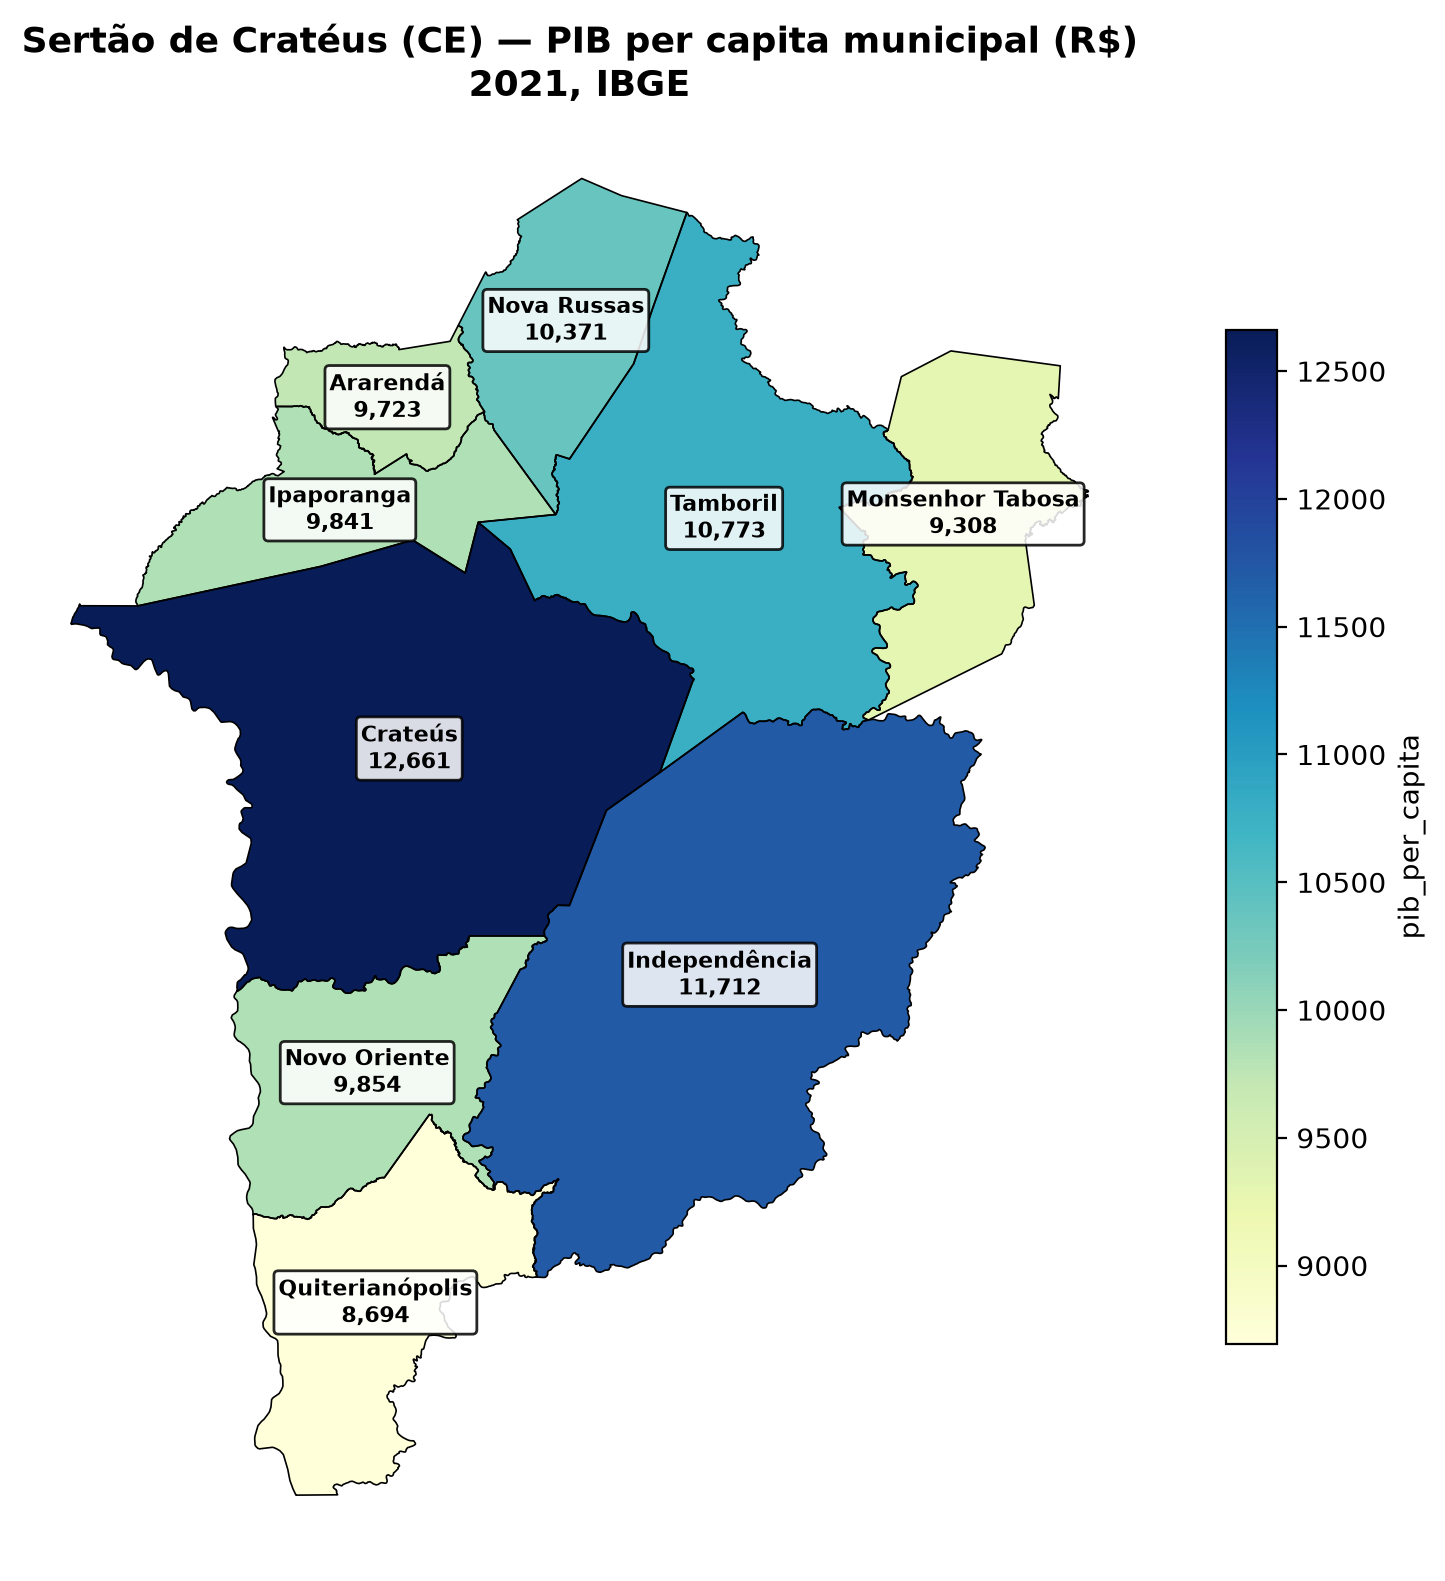
\includegraphics[width=0.78\textwidth]{../outputs/mapas/mapa_pib_per_capita_2021.png}
\caption{PIB per capita por município (2021, IBGE).}
\end{figure}

\section{Discussão}

Os resultados indicam que, no Sertão de Cratéus, a associação entre renda e desempenho escolar é \textbf{transversal, não temporal}: municípios com maior PIB per capita tendem a ter IDEB mais alto ($r = 0{,}49$; Figura 1), mas a variação temporal da renda não acompanha a variação do desempenho escolar (primeiras diferenças nulas; efeitos fixos não significativos; Figuras 2 e 3). A validação cruzada por município (Figura 3) sugere que a associação transversal é robusta e generalizada, não dependendo de um único município.

Dois pontos merecem destaque. Primeiro, a associação transversal não deve ser lida como ``a pobreza determina o baixo desempenho'': municípios pobres da microrregião alcançaram IDEB 2025 elevado (até 9,9 pontos), consistentemente acima da meta. Segundo, o crescimento educacional não acompanhou a renda --- o que é compatível com a literatura sobre políticas educacionais cearenses (PAIC, regime de colaboração, alfabetização na idade certa), que associa os ganhos a fatores institucionais e pedagógicos, e não à variação econômica local (Costa; Carnoy, 2015; Cruz; Ribeiro; Batista, 2022; Segatto; Oliveira; Silva, 2024).

As limitações são explícitas: (i) n municipal de 9 e 108 observações implica poder estatístico baixo (MDES de 5,71 com erro clusterizado), tornando a ausência de associação temporal uma \textbf{não-detecção} e não uma prova de ausência; (ii) o PIB municipal e a renda do responsável são proxies do desenvolvimento local --- o IPCE original não é auditável; (iii) não há pretensão causal; (iv) os efeitos fixos controlam fatores invariantes no tempo e choques comuns por ano, mas não outros confundidores variáveis; (v) as correlações transversais podem refletir fatores omitidos (infraestrutura, gestão) correlacionados com renda e desempenho.

\section{Considerações finais}

Este estudo responde à pergunta de pesquisa com evidência associativa subnacional: no Sertão de Cratéus, a relação entre renda e desempenho escolar é \textbf{transversal, não temporal} --- existe associação entre municípios (níveis), mas não dentro dos municípios ao longo do tempo. Adicionalmente, os dados oficiais mais recentes refutam a premissa de estagnação: todos os nove municípios superaram as metas pactuadas, com ganhos médios de cerca de seis pontos no período 2007--2025 e IDEB 2025 elevado mesmo em municípios de baixa renda. A ausência de associação temporal entre ganho educacional e renda sugere que fatores de política educacional --- e não a variação econômica --- estão associados à trajetória observada, em linha com a literatura do Ceará. Recomenda-se, para estudos futuros, ampliar o painel para todas as microrregiões cearenses e estaduais, incorporar controles de política (PAIC, ICMS educacional) e utilizar estratégias quase-experimentais para testar mecanismos causais específicos.

\section*{Referências}

{\sloppy
\noindent AFONSO, A. J. Para uma concetualização alternativa de accountability em educação. \textit{Educação \& Sociedade}, Campinas, v. 33, n. 119, p. 471--484, 2012. \href{https://doi.org/10.1590/S0101-73302012000200008}{https://doi.org/10.1590/S0101-73302012000200008}

\noindent ANDREWS, C. W.; VRIES, M. S. de. Pobreza e municipalização da educação: análise dos resultados do IDEB (2005-2009). \textit{Cadernos de Pesquisa}, São Paulo, v. 42, n. 147, p. 826--847, 2012. \href{https://doi.org/10.1590/S0100-15742012000300010}{https://doi.org/10.1590/S0100-15742012000300010}

\noindent BRUNELLO, G.; KISS, D. Math scores in high stakes grades. \textit{Economics of Education Review}, v. 87, 102219, 2022. \href{https://doi.org/10.1016/j.econedurev.2021.102219}{https://doi.org/10.1016/j.econedurev.2021.102219}

\noindent CARNOY, M.; MAROTTA, L.; LOUZANO, P.; et al. Intranational comparative education: what state differences in student achievement can teach us about improving education --- the case of Brazil. \textit{Comparative Education Review}, v. 61, n. 4, 2017. \href{https://doi.org/10.1086/693981}{https://doi.org/10.1086/693981}

\noindent CITO, L.; MARÔCO, J. Beyond the average: mapping educational inequality in Brazil with PISA 2022. \textit{Large-scale Assessments in Education}, v. 14, 2026. \href{https://doi.org/10.1186/s40536-026-00302-0}{https://doi.org/10.1186/s40536-026-00302-0}

\noindent COSTA, L. O.; CARNOY, M. The effectiveness of an early-grade literacy intervention on the cognitive achievement of Brazilian students. \textit{Educational Evaluation and Policy Analysis}, v. 37, n. 4, p. 567--590, 2015. \href{https://doi.org/10.3102/0162373715571437}{https://doi.org/10.3102/0162373715571437}

\noindent CRUZ, M. C. M. T.; RIBEIRO, V. M.; BATISTA, J. M. Contexto de implementação do Programa de Aprendizagem na Idade Certa (PAIC). \textit{Revista Ibero-Americana de Estudos em Educação}, Araraquara, v. 17, n. esp. 3, p. 2405--2432, 2022. \href{https://doi.org/10.21723/riaee.v17iesp.3.16719}{https://doi.org/10.21723/riaee.v17iesp.3.16719}

\noindent DUARTE, N. de S. O impacto da pobreza no Ideb: um estudo multinível. \textit{Revista Brasileira de Estudos Pedagógicos}, Brasília, DF, v. 94, n. 237, p. 343--363, 2013. \href{https://doi.org/10.1590/S2176-66812013000200002}{https://doi.org/10.1590/S2176-66812013000200002}

\noindent HANUSHEK, E. A.; WOESSMANN, L. \textit{The Knowledge Capital of Nations}: education and the economics of growth. Cambridge, MA: MIT Press, 2015. \href{https://doi.org/10.7551/mitpress/9780262029179.001.0001}{https://doi.org/10.7551/mitpress/9780262029179.001.0001}

\noindent LACRUZ, A. J.; AMÉRICO, B. L.; CARNIEL, F. Indicadores de qualidade na educação: análise discriminante dos desempenhos na Prova Brasil. \textit{Revista Brasileira de Estudos Pedagógicos}, Brasília, DF, v. 100, n. 254, 2019. \href{https://doi.org/10.1590/S1413-24782019240002}{https://doi.org/10.1590/S1413-24782019240002}

\noindent SCHNEIDER, M. P.; NARDI, E. L. O IDEB e a construção de um modelo de accountability na educação básica brasileira. \textit{Revista Portuguesa de Educação}, Braga, v. 27, n. 1, p. 7--28, 2014. \href{https://doi.org/10.21814/rpe.4295}{https://doi.org/10.21814/rpe.4295}

\noindent SEGATTO, C. I.; OLIVEIRA, K. de; SILVA, A. L. N. da. Os limites do PNE (2014-2024) no regime de colaboração. \textit{Estudos em Avaliação Educacional}, São Paulo, v. 35, e10549, 2024. \href{https://doi.org/10.18222/eae.v35.10549}{https://doi.org/10.18222/eae.v35.10549}

\noindent SOARES, J. F.; XAVIER, F. P. Pressupostos educacionais e estatísticos do Ideb. \textit{Educação \& Sociedade}, Campinas, v. 34, n. 124, p. 903--923, 2013. \href{https://doi.org/10.1590/S0101-73302013000300013}{https://doi.org/10.1590/S0101-73302013000300013}

\section*{Apêndice A --- Proveniência e reprodutibilidade}

{\sloppy
\noindent Scripts: \texttt{scripts/baixar\_dados.py}, \texttt{scripts/analise\_crateus.py}, \texttt{scripts/mapa\_crateus.py}, \texttt{scripts/graficos\_crateus.py}. Manifesto de fontes (URL, timestamp, SHA-256): \texttt{data/raw/SOURCE\_MANIFEST.json}. Resultados completos: \texttt{outputs/expanded/resultados\_r426.json}; proveniência computacional: \texttt{outputs/expanded/provenance\_r426.json}. Figuras: \texttt{outputs/figuras/} (scatter de níveis, séries temporais, LOOCV, ganho$\times$renda) e \texttt{outputs/mapas/} (renda do responsável, PIB per capita).

\noindent Declaração de limites: evidência associativa; n municipal de 9; MDES 5,71 (cluster); não-detecção declarada; IPCE substituído por proxies oficiais.}

\end{document}
